% \documentclass{article}
% \usepackage{xeCJK}
% \usepackage{tikz}
% \usetikzlibrary{decorations.pathreplacing, calligraphy}
% \usetikzlibrary{quotes,angles}
% \begin{document}
\begin{tikzpicture}
    \node at (1.1,-1.3) {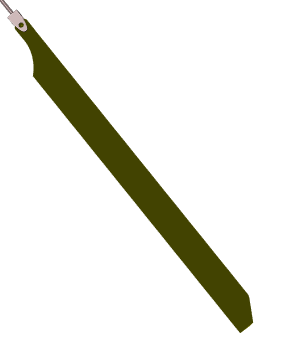
\includegraphics[width = 2.2cm]{blade.png}};
    \draw[dash dot](-2,0)--(1,0);
    \draw[dash dot](0,-2)--(0,1);
    \draw[-latex] -> (0,0)--(0,-3.0) node[left]{$X_h$};
    \draw[-latex] -> (0,0)--(1.8,0) node[above]{$Y_h$};
    \draw[-latex] -> (0,0)--(2.14,-2.7) node[left]{$X_r$};
    \draw[-latex] -> (0,0)--(1.5,1.1) node[above]{$Y_r$};
    \draw 
    (0,-4)coordinate(a)
    (0,0)coordinate(b)
    (2.14,-2.7)coordinate(c)
    pic["$\psi_r$", draw=orange, ->, angle eccentricity=1.2, angle radius=1.5cm]
    {angle=a--b--c};

\end{tikzpicture}  

% \end{document}